\documentclass{article}
\usepackage{amsmath}
\usepackage{amsfonts}
\usepackage{tikz}
\begin{document}
	
	\title{MATH6005 Assignment 3 Solutions}
	\author{Student Name}
	\date{October 2024}
	\maketitle
	
	\section*{Question 1}
	
	\subsection*{Part A: Independence of Random Variables}
	Consider a probability experiment in which a six-sided die is rolled. The outcome is represented by the set $ S = \{1, 2, 3, 4, 5, 6\} $. Let the random variables $ X, Y, Z : S \to \{0, 1, 2, 3\} $ be defined as follows:
	\[
	X(s) = s \mod 2, \quad Y(s) = s \mod 4, \quad Z(s) = 
	\begin{cases}
		0 & \text{if } s \leq 4, \\
		1 & \text{otherwise}.
	\end{cases}
	\]
	
	\subsection*{Answer:}
	
	
	\subsection*{Part B: Probability Calculation Using Bayes' Theorem}
	The mechanic reads the following from the manual:
	\begin{quote}
		``When the FCD warning light is illuminated and will not turn off, 90\% of the time the cause is a faulty wire, and the other 10\% of the time the cause is a faulty front collision sensor.''
	\end{quote}
	
	The diagnostic test results in either ``Fault Found'' or ``No Fault Found''. The test's accuracy is as follows:
	\begin{itemize}
		\item If the sensor is faulty, the test reports ``Fault Found'' 94\% of the time.
		\item If the sensor is not faulty, the test reports ``Fault Found'' 4\% of the time.
	\end{itemize}
	
	Using Bayes' theorem, calculate the probability that the sensor is faulty given that the test displays ``Fault Found''.
	
	Let:
	\begin{itemize}
		\item $ A $: The event that the sensor is faulty.
		\item $ B $: The event that the test reports ``Fault Found''.
	\end{itemize}
	
	Given:
	\[P(A) = 0.1, \quad P(\neg A) = 0.9\]
	\[P(B \mid A) = 0.94, \quad P(B \mid \neg A) = 0.04\]
	
	Using Bayes' theorem:
	\[P(A \mid B) = \frac{P(B \mid A) P(A)}{P(B)}\]
	where
	\[P(B) = P(B \mid A) P(A) + P(B \mid \neg A) P(\neg A)\]
	
	Substituting the values:
	\[P(B) = (0.94 \times 0.1) + (0.04 \times 0.9) = 0.094 + 0.036 = 0.13\]
	\[P(A \mid B) = \frac{0.94 \times 0.1}{0.13} \approx 0.723\]
	
	Thus, the probability that the sensor is faulty given that the test displays ``Fault Found'' is approximately 0.723.
	
	\section*{Question 2}
	
	\subsection*{Part A: Markov Process Model}
	To model the social mobility over many generations, a Markov process is used. The states of the Markov process are defined as follows:
	\begin{itemize}
		\item $S_1$: Service Sector
		\item $S_2$: Intermediate Sector
		\item $S_3$: Working Class Sector
		\item $S_4$: Farm Sector
	\end{itemize}
	The time steps represent the movement from father to son across generations.
	
	Assumptions:
	\begin{itemize}
		\item Employment transition probabilities depend only on the father's employment (i.e., memoryless property).
		\item Transitions are independent across families.
	\end{itemize}
	
	\subsection*{Part B: Transition Diagram and Matrix}
	The transition diagram is represented by the following directed graph:
	
	\begin{center}
		\begin{tikzpicture}[->, >=stealth', shorten >=1pt, auto, node distance=3cm, thick, main node/.style={circle, draw}]
			\node[main node] (S1) {Service};
			\node[main node] (S2) [below left of=S1] {Intermediate};
			\node[main node] (S3) [below right of=S1] {Working Class};
			\node[main node] (S4) [below of=S2] {Farm};
			
			\path[every node/.style={font=\small}]
			(S1) edge [bend left] node {0.32} (S2)
			edge [bend right] node {0.17} (S3)
			edge [loop above] node {0.64} (S1)
			edge node {0.13} (S4)
			(S2) edge node {0.36} (S2)
			edge node {0.22} (S1)
			edge node {0.27} (S3)
			edge node {0.21} (S4)
			(S3) edge node {0.55} (S3)
			edge node {0.31} (S2)
			edge node {0.13} (S1)
			edge node {0.34} (S4)
			(S4) edge [loop below] node {0.32} (S4);
		\end{tikzpicture}
	\end{center}
	
	The transition matrix $ T $ is:
	\[T = \begin{bmatrix}
		0.64 & 0.32 & 0.17 & 0.13 \\
		0.22 & 0.36 & 0.27 & 0.21 \\
		0.13 & 0.31 & 0.55 & 0.34 \\
		0.01 & 0.01 & 0.01 & 0.32
	\end{bmatrix}\]
	
	\subsection*{Part C: Calculation of $T^{10}$, $T^{100}$, and Prediction of Steady State}
	Using a computer program such as Reshish Matrix Calculator, the following matrices are calculated:
	\[T^{10} = \ldots, \quad T^{100} = \ldots\]
	The steady state appears to converge to a vector $\pi$, suggesting the long-term probabilities of employment across the sectors.
	
	\subsection*{Part D: Finding Steady State Vector}
	The steady state vector $\pi$ is found using the shortcut method. Solve:
	\[\pi T = \pi, \quad \text{subject to } \sum_i \pi_i = 1\]
	
	\subsection*{Part E: Long-term Distribution of Jobs}
	The steady state vector $\pi$ indicates the long-term distribution of jobs in England and Wales. It suggests that, over many generations, the proportion of individuals in each sector stabilizes to the values given by $\pi$.
	
	\section*{Question 3}
	
	\subsection*{Part A: Drawing Hypercube Graphs}
	The hypercube graphs for $ H_1, H_2, H_3, H_4 $ are drawn.
	
	\begin{center}
		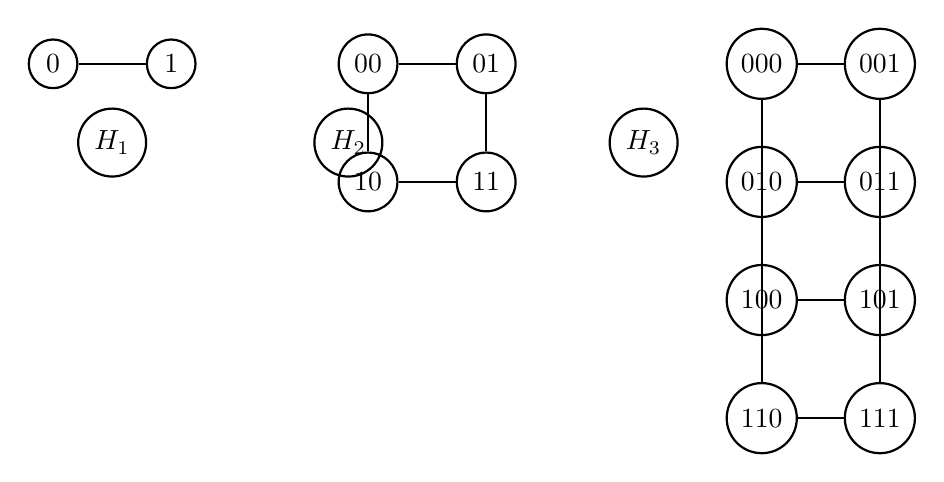
\begin{tikzpicture}[every node/.style={circle, draw}, node distance=1.5cm, thick]
			% H1
			\node (A) {0};
			\node (B) [right of=A] {1};
			\draw (A) -- (B);
			\node at (0.75, -1) {$H_1$};
			
			% H2
			\node (A1) [right of=B, xshift=1cm] {00};
			\node (B1) [right of=A1] {01};
			\node (C1) [below of=A1] {10};
			\node (D1) [below of=B1] {11};
			\draw (A1) -- (B1) -- (D1) -- (C1) -- (A1);
			\node at (3.75, -1) {$H_2$};
			
			% H3
			\node (A2) [right of=B1, xshift=2cm] {000};
			\node (B2) [right of=A2] {001};
			\node (C2) [below of=A2] {010};
			\node (D2) [below of=B2] {011};
			\node (E2) [below of=C2] {100};
			\node (F2) [below of=D2] {101};
			\node (G2) [below of=E2] {110};
			\node (H2) [below of=F2] {111};
			\draw (A2) -- (B2) -- (D2) -- (C2) -- (A2);
			\draw (E2) -- (F2) -- (H2) -- (G2) -- (E2);
			\draw (A2) -- (E2);
			\draw (B2) -- (F2);
			\draw (C2) -- (G2);
			\draw (D2) -- (H2);
			\node at (7.5, -1) {$H_3$};
		\end{tikzpicture}
	\end{center}
	
	\subsection*{Part B: Diagnostic Test Feasibility}
	The diagnostics consultant requires that the first cable tested is adjacent to the CPU associated with the binary string of $ n $ zeroes, and that each subsequent cable connects to the same CPU as the previous one, with each cable tested exactly once.
	
	To determine if this testing procedure is feasible, it is necessary to determine if an Eulerian path exists in $ H_n $. An Eulerian path exists if there are exactly zero or two vertices of odd degree. Since each vertex in a hypercube graph has even degree, an Eulerian path exists, and thus the proposed arrangement allows for the diagnostics tests to be run as required.
	
	\subsection*{Part C: Budget Calculation}
	The budget for constructing the network is \$700,000. Each cable costs \$100 and each CPU costs \$1000.
	
	The number of vertices (CPUs) in $ H_n $ is $ 2^n $, and the number of edges (cables) is $ n \times 2^{n-1} $. The total cost $ C(n) $ is:
	\[C(n) = 1000 \times 2^n + 100 \times n \times 2^{n-1}\]
	
	Determine the largest value of $ n $ for which $ C(n) \leq 700,000 $:
	\[C(n) = 1000 \times 2^n + 100 \times n \times 2^{n-1} \leq 700,000\]
	
	Using trial and error or a computer to solve, the maximum value of $ n $ that satisfies this condition is $ n = 6 $.
	
	\section*{Question 4}
	
	\subsection*{Part A: Proof of (1) $\implies$ (2)}
	If $ T $ is a tree, then it has no simple circuits and $ n - 1 $ edges.
	
	\textbf{Proof by induction on the number of vertices $|V(T)|$.}
	
	\textbf{Base case:} Let $|V(T)| = 1$. A tree with only one vertex has no edges and no circuits, so the statement holds.
	
	\textbf{Inductive step:} Assume that the statement is true for a tree with $ n $ vertices. Now consider a tree $ T' $ with $ n + 1 $ vertices. By Lemma 1, $ T' $ has at least one leaf, say $ v $. Removing $ v $ from $ T' $ results in a tree $ T $ with $ n $ vertices, which by the inductive hypothesis has $ n - 1 $ edges. Since adding the leaf $ v $ adds exactly one edge, $ T' $ has $ (n - 1) + 1 = n $ edges, and no circuits. Thus, the statement holds for $ n + 1 $, completing the proof.
	
	\subsection*{Part B: Logical Equivalence of Statements}
	The following six statements about a graph $ T $ are given:
	\begin{enumerate}
		\item $ T $ is a tree.
		\item $ T $ has no simple circuits and $ n - 1 $ edges.
		\item $ T $ is connected and has $ n - 1 $ edges.
		\item $ T $ is connected and every edge is a bridge.
		\item Any two vertices of $ T $ are connected by exactly one simple path.
		\item $ T $ contains no non-trivial circuits, but the addition of any new edge that connects an existing pair of vertices will create a simple circuit.
	\end{enumerate}
	
	To prove Theorem 2, all six statements must be shown to be logically equivalent. If it can be proven that:
	\[(1) \implies (2), (2) \implies (3), (3) \implies (4), (4) \implies (5), (5) \implies (6), (6) \implies (1)\]
	then each statement is equivalent to the others, and Theorem 2 is proved.
	
	\subsection*{Part C: Missing Statement in Set $ T $}
	The following implications have been proven:
	\[T = \{(1) \implies (2), (5) \implies (3), (6) \implies (5), (2) \implies (4), (3) \implies (1)\}\]
	
	To complete the proof of Theorem 2, an additional implication $(i, j)$ must be found to make the set $ T \cup \{(i) \implies (j)\} $ sufficient to prove the theorem.
	
	By examining the existing implications, it is evident that there is no direct proof between statements (4) and (6). Thus, adding $(4) \implies (6)$ would complete the set and make $ T $ sufficient to prove Theorem 2.
	
	\subsection*{Part D: Proof that $ |E(G)| = |V(G)| - s $ for a Forest}
	Let $ G $ be a forest with $ s $ connected components.
	
	\textbf{Proof:}
	Assume $ G $ is a forest, which means it is a disjoint collection of trees. Let $ G $ have $ s $ connected components, which are trees. For each tree component $ T_i $, let $ |V(T_i)| = n_i $. Since $ T_i $ is a tree, it has $ n_i - 1 $ edges.
	
	The total number of vertices in $ G $ is:
	\[|V(G)| = \sum_{i=1}^{s} n_i\]
	The total number of edges in $ G $ is:
	\[|E(G)| = \sum_{i=1}^{s} (n_i - 1) = \left( \sum_{i=1}^{s} n_i \right) - s = |V(G)| - s\]
	
	Thus, $ |E(G)| = |V(G)| - s $, as required.
	
\end{document}
